%\ifx\wholebook\relax\else
%\documentclass[twoside]{book}
%\usepackage[active]{srcltx}
%\usepackage[LY1]{fontenc}
%\usepackage{url}
\makeatletter
\def\url@leostyle{%
  \@ifundefined{selectfont}{\def\UrlFont{\sf}}{\def\UrlFont{\sffamily}}}
\makeatother
% Now actually use the newly defined style.
\urlstyle{leo}

\usepackage{graphicx}
\def\etc{{\textit etc}}
\def\eg{{\textit e.g.}}
\def\ie{{\textit i.e.}}
\def\cf{{\textit c.f.}\ }
\def\erf{\mathop{\textrm erf}}
\def\sign{\mathop{\textrm sign}}
\def\prob{\mathop{\textrm Prob}}
\def\var{\mathop{\textrm var}}
\def\mod{\mathop{\textrm mod}}
\def\cor{\mathop{\textrm cor}}
\def\cov{\mathop{\textrm cov}}
\def\cl{\mathop{\textrm CL}}
\def\kg{\mathop{\textrm Kg}}
\def\patstyle#1{{\textsc #1}}
\def\th{^{\mathop{\textrm th}}}
%\def\st#1{^{\mathop{\rm #1}}}
\def\note#1{\begin{quote}{\textbf Note:} #1\end{quote}}
\def\braket#1{\left\langle #1\right\rangle}
\def\order#1{\let\o=#1{\cal O}\ifx\o 1$\left(n\right)$\else$\left(n^{#1}\right)$\fi}
%\newtheorem{privListing}{Listing}[chapter]
%\newenvironment{listing}{\vskip 3ex\hrule\vskip 1ex\begin{privListing}}{\end{privListing}\hrule\vskip 1ex}
\newtheorem{privExample}{Code example}[chapter]
\newenvironment{codeExample}{\begin{privExample}\begin{quote}\tt}{\end{quote}\end{privExample}}
\def\relboxl#1#2{\hbox to #1\hsize{#2\hfil}}
\def\relboxc#1#2{\hbox to #1\hsize{\hfil #2\hfil}}
\def\relboxr#1#2{\hbox to #1\hsize{\hfil #2}}
\def\transpose#1{{\bf #1}^{\mathop{\rm T}}}
\def\inverse#1{{\bf #1}^{-1}}
%\def\tm{$^{\mathop{\rm TM}}$}
\def\tm{ }
\newenvironment{mainEquation}{\marginpar[\vspace{3 ex} Main
equation$\Rightarrow$]{\vspace{3 ex}$\Leftarrow$Main
equation}\begin{equation}}{\end{equation}}
\def\rubrique#1{\paragraph{#1}\hfil\par\noindent}

%\begin{document}
%\fi

\chapter{Interpolation}
\label{ch:interpolation}
\begin{flushright}
{\textsl On ne peut pr\'evoir les choses qu'apr\`es qu'elles sont
arriv\'ees.}\footnote{One can predict things only after they have
occurred.}\\ Eug\`ene Ionesco
\end{flushright}
\vspace{1 ex} Interpolation is a technique allowing the estimation
of a function over the range covered by a set of points at which
the function's values are known. These points are called the {\textsl
sample} points. Interpolation is useful to compute a function
whose evaluation is highly time consuming: with interpolation it
suffices to compute the function's values for a small number of
well-chosen sample points. Then, evaluation of the function
between the sample points can be made with interpolation.

Interpolation can also be used to compute the value of the inverse
function, that is finding a value $x$ such that
$f\left(x\right)=c$ where $c$ is a given number, when the function
is known for a few sample points bracketing the sought value.
People often overlook this easy and direct computation of the
inverse function.

Interpolation is often used interchangeably with extrapolation.
This is not correct, however. Extrapolation is the task of
estimating a function outside of the range covered by the sample
points. If no model exists for the data extrapolation is just
gambling. Methods exposed in this chapter should not be used for
extrapolation.

Interpolation should not be mistaken with function (or curve)
fitting. In the case of interpolation the sample points purely
determine the interpolated function. Function fitting allows
constraining the fitted function independently from the sample
points. As a result fitted functions are more stable than
interpolated functions especially when the supplied values are
subject to fluctuations coming from rounding or measurement
errors. Fitting is discussed in chapter \ref{ch:estimation}.

\section{General remarks}
\label{sec:interpolgen} There are several methods of
interpolation. One difference is the type of function used. The
other is the particular algorithm used to determine the function.
For example, if the function is periodic, interpolation can be
obtained by computing a sufficient number of coefficients of the
Fourier series for that function.

In the absence of any information about the function, polynomial
interpolation gives fair results. The function should not have any
singularities over the range of interpolation. In addition there
should not be any pole in the vicinity of the complex plane near
the portion of the real axis corresponding to the range of
interpolation. If the function has singularities it is recommended
to use rational functions --- that is the quotient of two
polynomials --- instead \cite{Press}.

In this chapter we discuss 3 interpolation functions: Lagrange
interpolation polynomial, a diagonal rational function
(Bulirsch-Stoer interpolation) and cubic spline. Furhermore, we
show 3 different implementation of the Lagrange interpolation
polynomial: direct implementation of Lagrange's formula, Newton's
algorithm and Neville's algorithm.
\begin{figure}
\label{cls:interpolation}
\centering\includegraphics[width=11cm]{Figures/InterpolationClassDiagram}
\caption{Class diagram for the interpolation classes}
\end{figure}
Figure \ref{cls:interpolation} shows how the classes corresponding
to the different interpolation methods described in this chapter
are related to each other.

\rubrique{Definition} The {\textit Lagrange interpolation polynomial}
is the unique polynomial of minimum degree going through the
sample points. The degree of the polynomial is equal to the number
of supplied points minus one. A diagonal rational function is the
quotient of two polynomials where the degree of the polynomial in
the numerator is at most equal to that of the denominator. Cubic
spline uses piece-wise interpolation with polynomials but limits
the degree of each polynomial to 3 (hence the adjective cubic).

\rubrique{Examples} Before selecting an interpolation method the
user must investigate the validity of the interpolated function
over the range of its intended use. Let us illustrate this remark
with an example from high-energy physics, that, in addition, will
expose the limitation of the methods exposed in this chapter.

\begin{figure}
\label{fig:landauinterpol}
\centering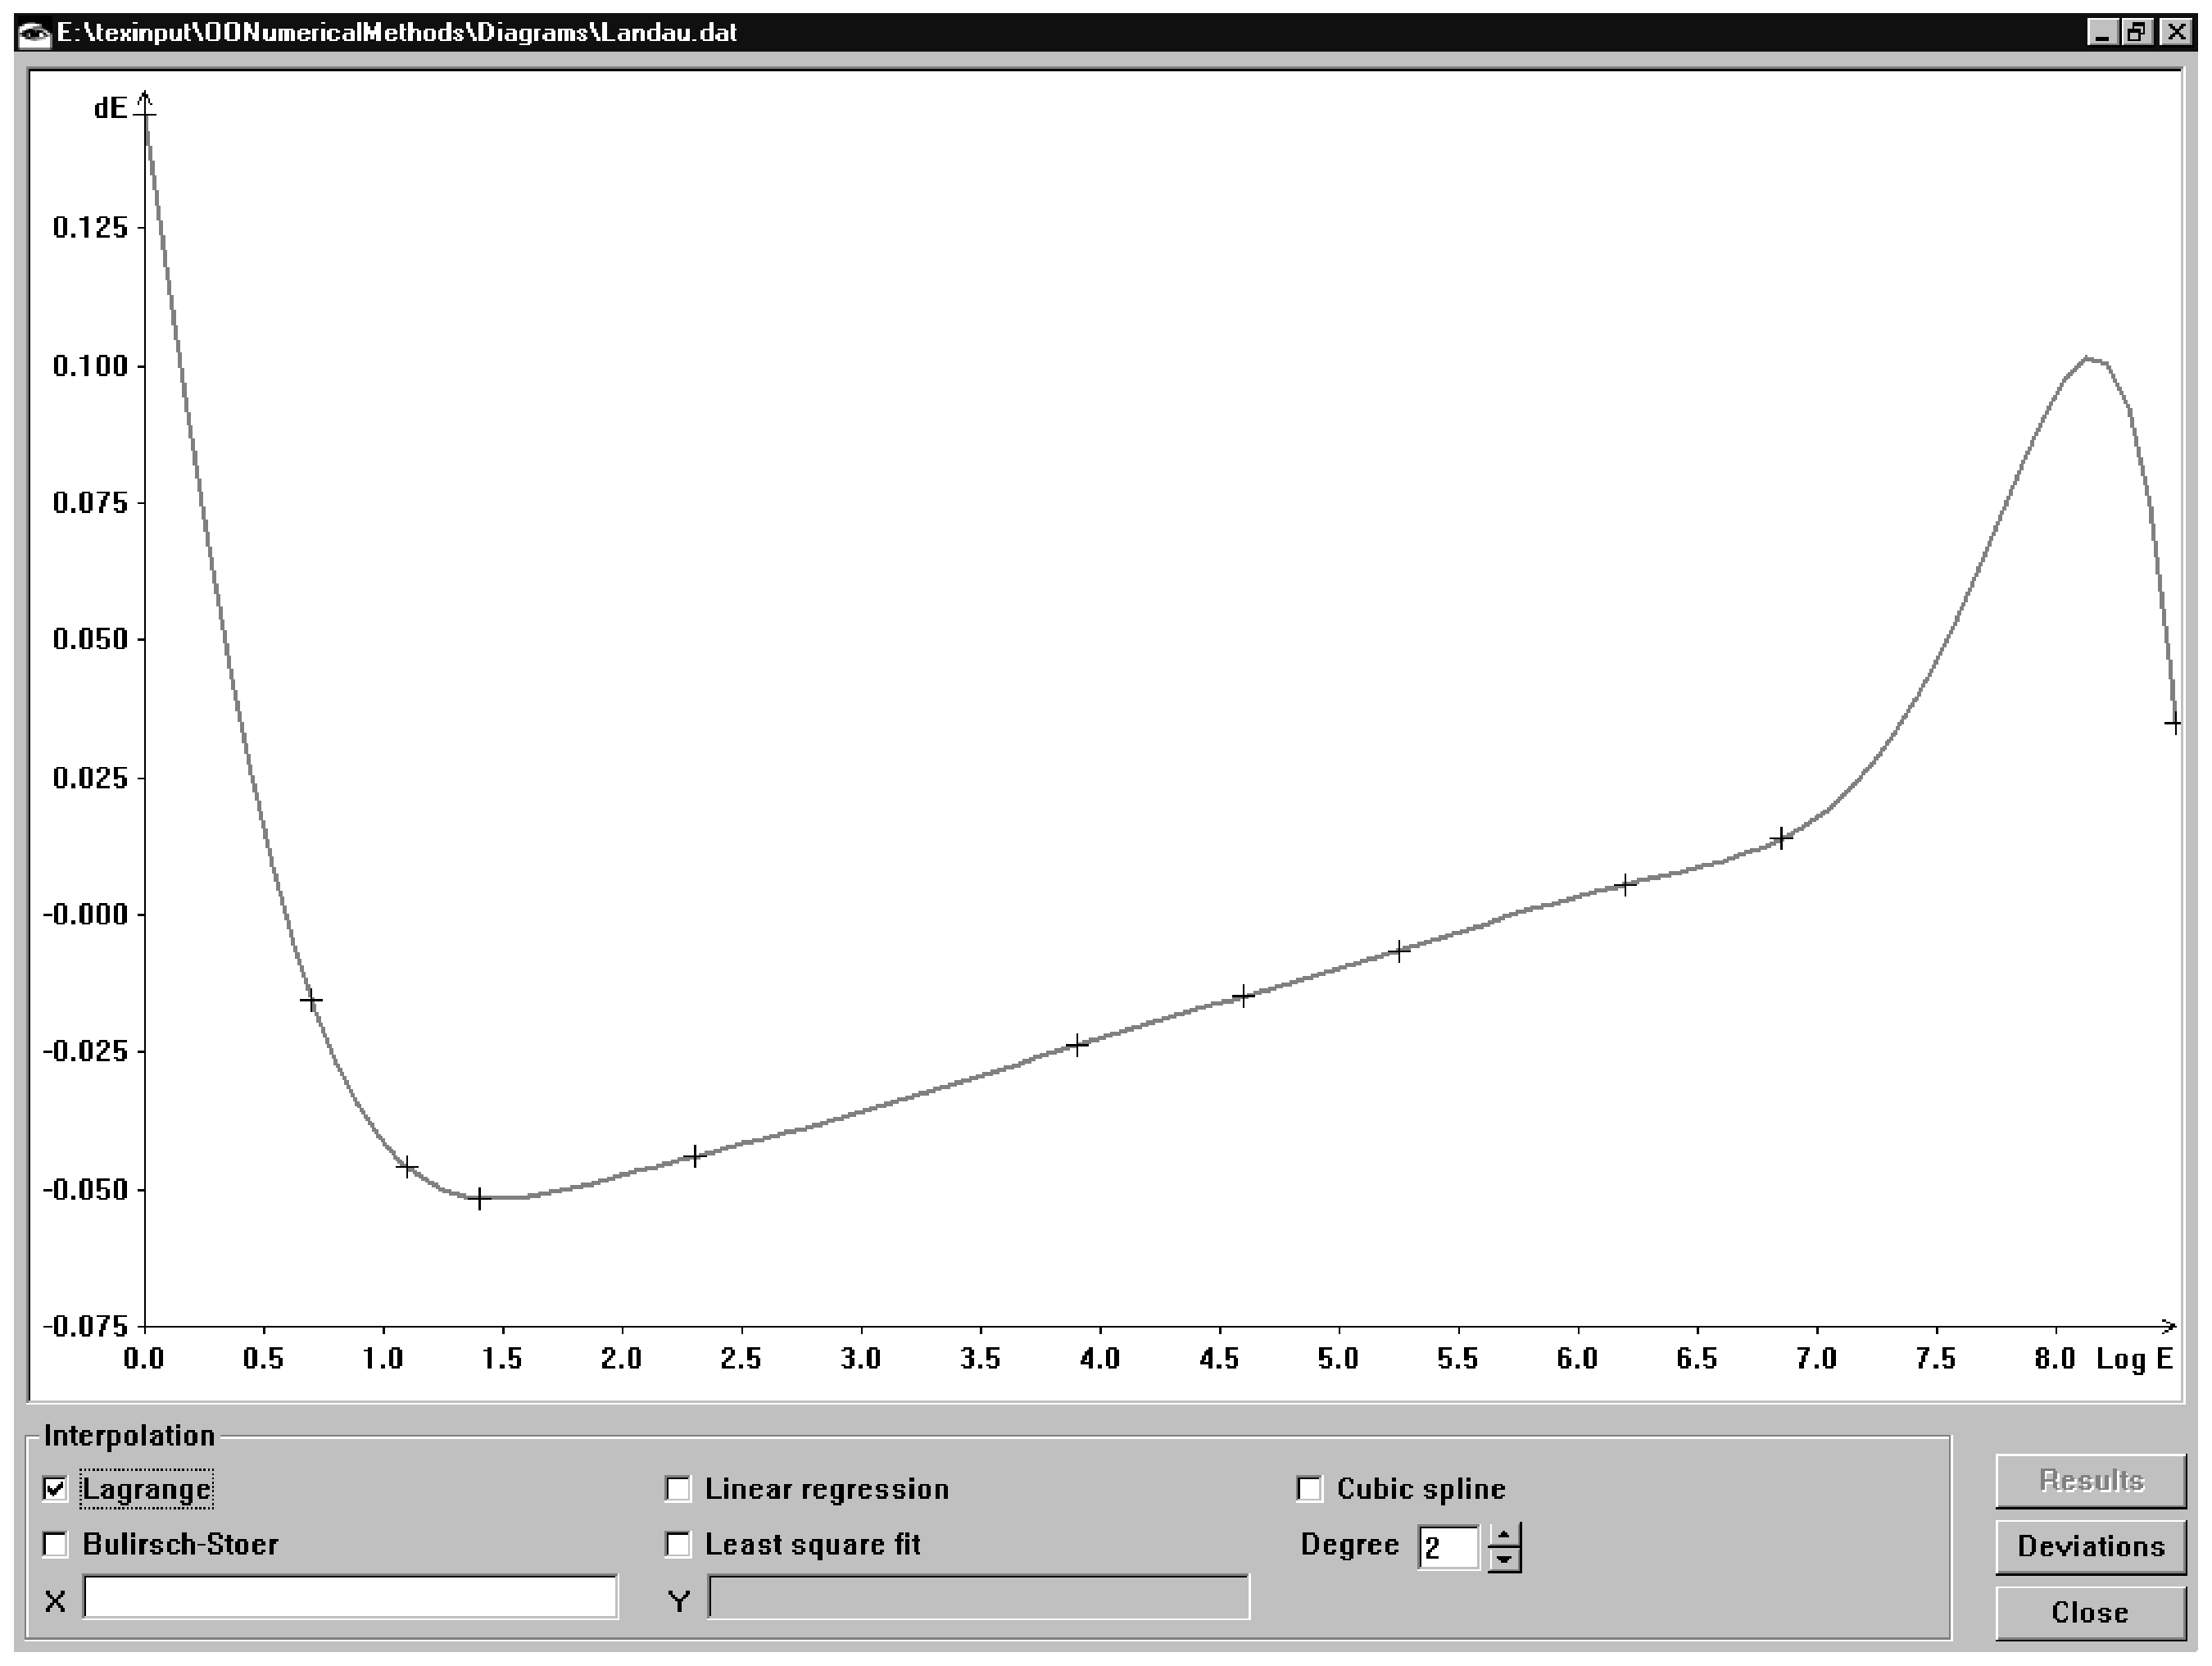
\includegraphics[width=12cm]{Figures/Lagrange}
\caption{Example of interpolation with the Lagrange interpolation
polynomial}
\end{figure}
Figure \ref{fig:landauinterpol} shows sample points --- indicated
by crosses --- representing correction to the energy measured
within a gamma ray detector made of several densely packed
crystals. The energy is plotted on a logarithmic scale. The
correction is caused by the absorption of energy in the wrapping
of each crystal. The sample points were computed using a
simulation program\footnote{This program - EGS written by Ralph
Nelson of the Stanford Linear Accelerator Center (SLAC) -
simulates the absorption of electromagnetic showers inside matter.
Besides being used in high-energy physics this program is also
used in radiology to dimension detectors of PET scanners and other
similar radiology equipment.}, each point requiring several hours
of computing time. Interpolation over these points was therefore
used to allow a quick computation of the correction at any energy.
This is the main point of this example: the determination of each
point was expensive in terms of computing time, but the function
represented by these points is continuous enough to be
interpolated. The simulation program yields results with good
precision so that the resulting data are not subjected to
fluctuation.

The gray thick line in figure \ref{fig:landauinterpol} shows the
Lagrange interpolation polynomial obtained from the sample points.
It readily shows limitations inherent to the use of interpolation
polynomials. The reader can see that for values above 6.5 ---
corresponding to an energy of 500 MeV --- the interpolated
function does not reproduce the curve corresponding to the sample
points. In fact, above 4.0 --- that is,  50 MeV on the scale of
figure \ref{fig:landauinterpol} --- the correction is expected to
be a linear function of the logarithm of the energy.

\begin{figure}
\label{fig:interpolex2}
\centering\includegraphics[width=12cm]{Figures/LagrangeVsRational}
\caption{Comparison between Lagrange interpolation and
interpolation with a rational function}
\end{figure}
Figure \ref{fig:interpolex2} shows a comparison between the
Lagrange interpolation polynomial (gray thick line) and
interpolation with a rational function (black dotted line) using
the same sample points as in figure \ref{fig:landauinterpol}. The
reader can see that, in the high-energy region (above 4 on the
scale of figure \ref{fig:interpolex2}) the rational function does
a better job than the Lagrange polynomial. Between the first two
points, however, the rational function fails to reproduce the
expected behavior.

\begin{figure}
\label{fig:interpolex3}
\centering\includegraphics[width=12cm]{Figures/LagrangeVsSpline}
\caption{Comparison of Lagrange interpolation and cubic spline}
\end{figure}
Figure \ref{fig:interpolex3} shows a comparison between the
Lagrange interpolation polynomial (gray thick line) and cubic
spline interpolation (black dotted line) using the same sample
points as in figure \ref{fig:landauinterpol}. The reader can see
that, in the high-energy region (above 4 on the scale of figure
\ref{fig:interpolex2}) the cubic spline does a better job than the
Lagrange polynomial. In fact, since the dependence is linear over
that range, the cubic spline reproduces the theoretical dependence
exactly. In the low energy region, however, cubic spline
interpolation fails to reproduce the curvature of the theoretical
function because of the limitation of the polynomial's degree.

A final example shows a case where interpolation should not be
used. Here the sample points represent the dependence of the
probability that a coin mechanism accepts a wrong coin as a
function of an adjustable threshold. The determination of each
point requires 5-10 minutes of computing time.
\begin{figure}
\label{fig:interpolex4}
\centering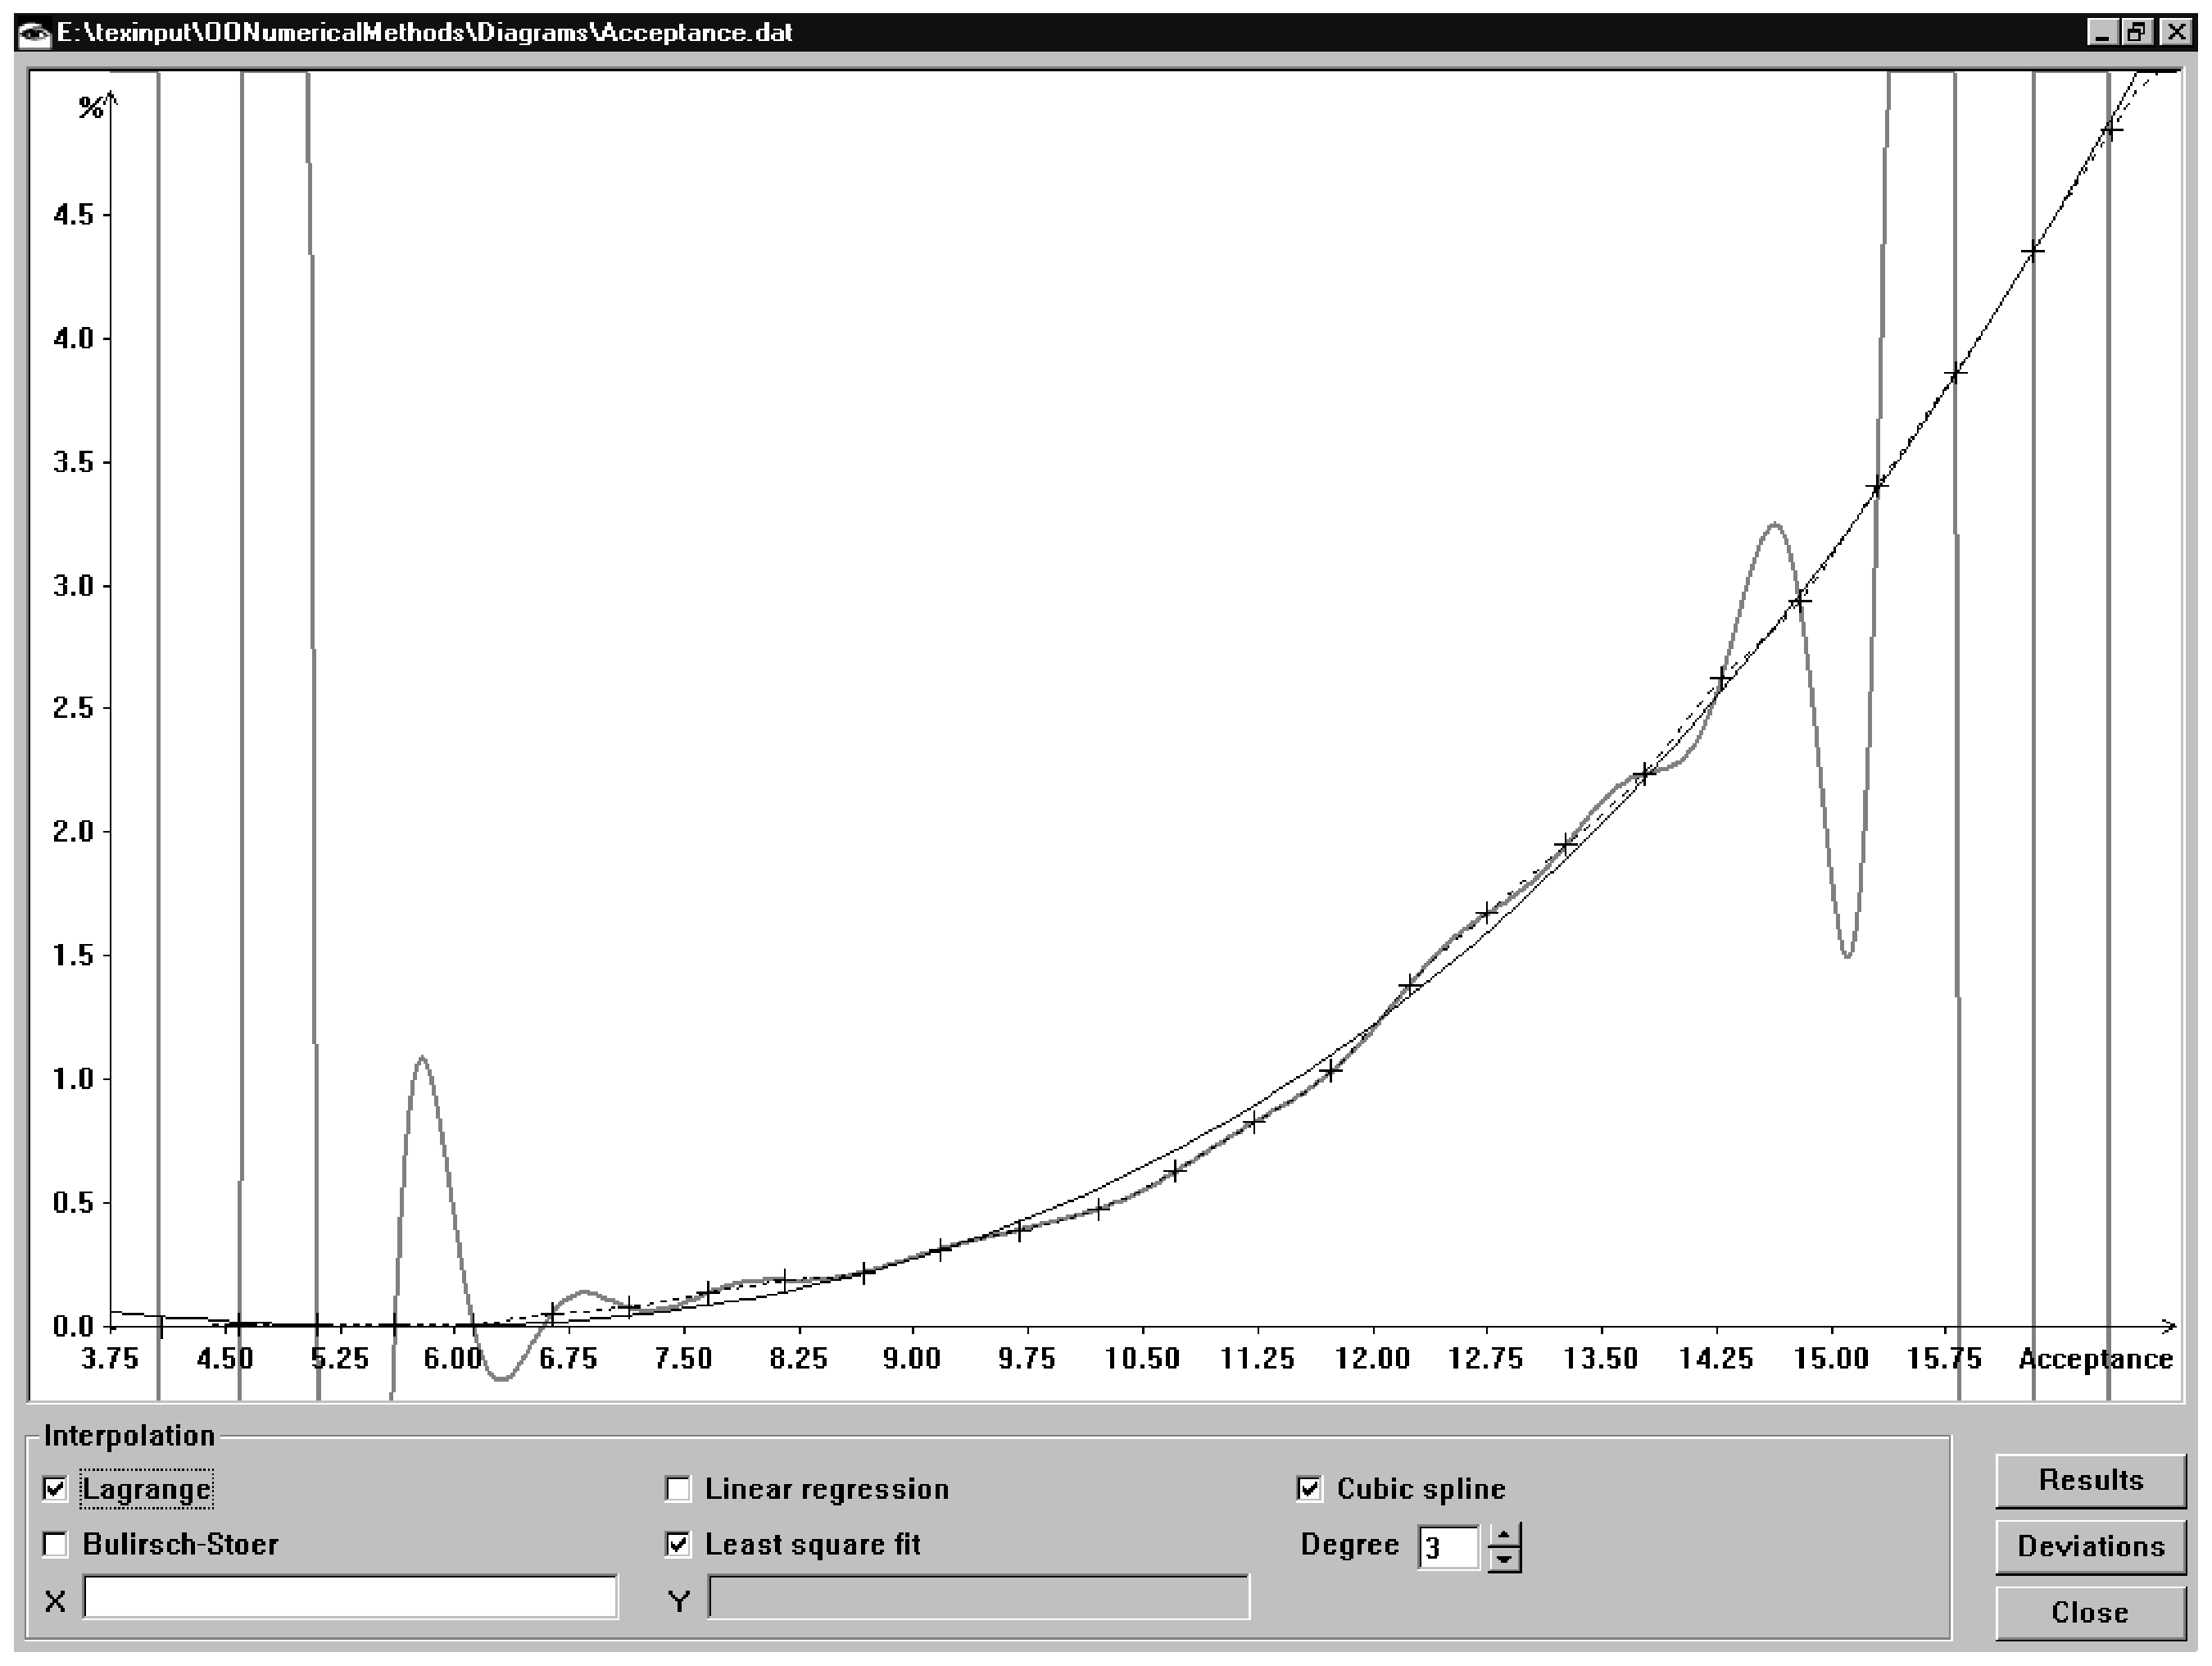
\includegraphics[width=12cm]{Figures/BadInterpolation}
\caption{Example of misbehaving interpolation}
\end{figure}
In this case, however, the simulation was based on using
experimental data. Contrary to the points of figure
\ref{fig:landauinterpol} the points of figure
\ref{fig:interpolex4} are subjected to large fluctuations, because
the sample points have been derived from measured data. Thus,
interpolation does not work.

As in figure \ref{fig:interpolex2}, the gray thick line is the
Lagrange interpolation polynomial and the black dotted line is the
cubic spline. Clearly the Lagrange interpolation polynomial is not
giving any reasonable interpolation. Cubic spline is not really
better as is tries very hard to reproduce the fluctuations of the
computed points. In this case, a polynomial fit (\cf section
\ref{sec:lsfpol}) is the best choice: the thin black line shows
the result of a fit with a $3^{rd}$ degree polynomial.
Another example of unstable interpolation is given in
section \ref{sec:lsfpol} (figure \ref{fig:femurLength}).

\rubrique{Three implementations of Lagrange interpolation} Once
you have verified that a Lagrange interpolation polynomial can be
used to perform reliable interpolation over the sample points, you
must chose among 3 algorithms to compute the Lagrange
interpolation polynomial: direct Lagrange formula, Newton's
algorithm and Neville's algorithm.

Newton's algorithm stores intermediate values which only depends
on the sample points. It is thus recommended, as it is the fastest
method to interpolate several values over the same sample points.
Newton's algorithm is the method of choice to compute a function
from tabulated values.

Neville's algorithm gives an estimate of the numerical error
obtained by the interpolation. It can be used when such
information is needed. Romberg integration, discussed in section
\ref{sec:romberg}, uses Neville's method for that reason.

\section{Lagrange interpolation}
\label{sec:lagrange}
 Let us assume a set of numbers
$x_0,\ldots,x_n$ and the corresponding function's values
$y_0,\ldots,y_n$. There exist a unique polynomial
$P_n\left(x\right)$ of degree $n$ such that
$P_n\left(x_i\right)=y_i$ for all $i=0,\ldots,n$. This polynomial
is the Lagrange interpolation polynomial whose expression is given
by \cite{Knuth2}:
\begin{equation}
\label{eq:lagrange} P_n\left(x\right)=\sum_{i=0}^n{\prod_{j\neq
i}\left(x-x_j\right) \over\prod_{j\neq i}\left(x_i-x_j\right)}y_i.
\end{equation}
For example, the Lagrange interpolation polynomial of degree 2 on
3 points is given by:
\begin{equation}
P_2\left(x\right)={\left(x-x_1\right)\left(x-x_2\right)\over
\left(x_0-x_1\right)\left(x_0-x_2\right)}y_0+{\left(x-x_0\right)\left(x-x_2\right)\over
\left(x_1-x_0\right)\left(x_1-x_2\right)}y_1+{\left(x-x_0\right)\left(x-x_1\right)\over
\left(x_2-x_0\right)\left(x_2-x_1\right)}y_2
\end{equation}

The computation of the polynomial occurs in the order of $\mathcal{O}(n^2)$ since it involves a double iteration.
One can save the evaluation of a few products by rewriting equation \ref{eq:lagrange} as:
\begin{equation}
\label{eq:lagrangesimp}
P_n\left(x\right)=\prod_{i=0}^n\left(x-x_i\right)\sum_{i=0}^n{y_i
\over\left(x-x_i\right)\prod_{j\neq i}\left(x_i-x_j\right)}.
\end{equation}
Of course, equation \ref{eq:lagrangesimp} cannot be evaluated at
the points defining the interpolation. This is easily solved by
returning the defining values as soon as one of the first products
becomes zero during the evaluation.

\subsection{Lagrange interpolation --- Smalltalk implementation}
%\label{sec:slagrange}\marginpar{Figure \ref{cls:interpolation} with the box {\textbf LagrangeInterpolator} grayed.}
The object responsible to implement Lagrange interpolation is defined
uniquely by the sample points over which the interpolation is
performed. In addition it should behave as a function. In other
words it should implement the behavior of a one-variable function
as discussed in section \ref{sec:stFunction}. For example linear
interpolation behaves as follows:

\begin{listing}[label=ex:lagrangeS1]{Smalltalk}
{Linear interpolation}
| interpolator |
interpolator := PMLagrangeInterpolator
                        points: (Array with: 1 @ 2
                                        with: 3 @ 1).
interpolator value: 2.2
\end{listing}

In this example, one creates a new instance of the class \code{PMLagrangeInterpolator} by sending the message \code{points:} to the class \code{PMLagrangeInterpolator} with the collection of
sample points as argument.
The newly created instance is stored in the variable \code{interpolator}.
The next line shows how to compute an interpolated value.

The creation method \code{points:} takes as argument the collection
of sample points. However, it could also accept any object
implementing a subset of the methods of the class \code{Collection}
--- namely the methods \code{size}, \code{at:} and, if we want to be
able to add new sample points, \code{add:}.

One can also spare the creation of an explicit collection object
by implementing these collection methods directly in the Lagrange
interpolation class.
Now, one can also perform interpolation in the following way:

\begin{listing}[label=ex:lagrangeS2]{Smalltalk}
{Alternate way to do a linear interpolation}
| interpolator deviation |
interpolator := PMLagrangeInterpolator new.
1 to: 45 by: 2 do:
                [ :x | interpolator add: x @ (x degreesToRadians sin)].
deviation := (interpolator value: 8) -(8 degreesToRadians sin).
\end{listing}

The code above creates an instance of the class \code{PMLagrangeInterpolator} with an empty collection of sample points. It then adds sample points one by one directly into the
interpolator object. Here the sample points are tabulated values
of the sine function for odd degree values between 1 and 45
degree. The final line of the code compares the interpolated value
with the correct one.

Listing \ref{lst:lagrange} shows the full code of the class
implementing the interface shown above.

The class \code{PMLagrangeInterpolator} is implemented with a
single instance variable containing the collection of sample
points. Each point contains a pair of values
$\left(x_i,y_i\right)$ and is implemented with object of the base
class \code{Point} since an instance of \code{Point} can contain any
type of object in its coordinates. There are two creation methods,
\code{points:} and \code{new}, depending on whether the sample
points are supplied as an explicit object or not. Each creation
method calls in turn an initialization method, respectively \code{initialize:} and \code{initialize}.

The method \code{points:} takes as argument the collection of the
sample points. This object must implement the following methods of
the class \code{Collection}: \code{size}, \code{at:} and \code{add:}.
If the class is created with the method \code{new} an implicit
collection object is created with the method \code{defaultSamplePoints}. This arrangement allows subclasses to select
another type of collection if needed. The default collection
behavior implemented by the class \code{PMLagrangeInterpolator} is
minimal, however. If there is a need for more flexible access to
the collection of sample points, a proper collection object or a
special purpose object should be used.

The interpolation itself is implemented within the single method
\code{value:}. This method is unusually long for object-oriented
programming standards. In this case, however, there is no
compelling reason to split any portion of the algorithm into a
separate method.
Moreover, splitting the method would increase the
computing time.

A final discussion should be made about the two methods \code{xPointAt:} and \code{yPointAt:}.
In principle, there is no need for these methods as the value could be grabbed directly from the collection of points.
If one needs to change the implementation of the point collection in a subclass, however, only these two methods need to be modified.
Introducing this kind of construct can go a long way in program maintenance.

\begin{listing}[label=lst:lagrange]{Smalltalk}
{Smalltalk implementation of the Lagrange interpolation}
Object subclass: #PMLagrangeInterpolator
   instanceVariableNames: 'pointCollection'
   classVariableNames: ''
   package: 'Math-DHB-Numerical-Math-Interpolator'
\end{listing}

\begin{displaycode}{Smalltalk}
PMLagrangeInterpolator class >> new
    ^super new initialize
\end{displaycode}

\begin{displaycode}{Smalltalk}
PMLagrangeInterpolator class >> points: aCollectionOfPoints
    ^self new initialize: aCollectionOfPoints
\end{displaycode}

\begin{displaycode}{Smalltalk}
PMLagrangeInterpolator add: aPoint
    ^pointCollection add: aPoint
\end{displaycode}

\begin{displaycode}{Smalltalk}
PMLagrangeInterpolator >> defaultSamplePoints
    ^OrderedCollection new
\end{displaycode}

\begin{displaycode}{Smalltalk}
PMLagrangeInterpolator >> initialize
    ^self initialize: self defaultSamplePoints
\end{displaycode}

\begin{displaycode}{Smalltalk}
PMLagrangeInterpolator >> initialize: aCollectionOfPoints
    pointCollection := aCollectionOfPoints.
    ^self
\end{displaycode}

\begin{displaycode}{Smalltalk}
PMLagrangeInterpolator >> value: aNumber
    | norm dx products answer size |
    norm := 1.
    size := pointCollection size.
    products := Array new: size.
    products atAllPut: 1.
    1 to: size
        do: [ :n |
              dx := aNumber - ( self xPointAt: n).
              dx = 0
                ifTrue: [ ^( self yPointAt: n)].
              norm := norm * dx.
              1 to: size
                do: [ :m |
                      m = n
                        ifFalse:[ products at: m put: ( (( self 
            xPointAt: m) - ( self xPointAt: n)) * ( products at: m))].
                    ].
            ].
    answer := 0.
    1 to: size do:
        [ :n | answer := ( self yPointAt: n) / ( ( products at: n) * 
                          ( aNumber - ( self xPointAt: n))) + answer].
    ^norm * answer
\end{displaycode}

\begin{displaycode}{Smalltalk}
PMLagrangeInterpolator >> xPointAt: anInteger
    ^( pointCollection at: anInteger) x
\end{displaycode}

\begin{displaycode}{Smalltalk}
PMLagrangeInterpolator >> yPointAt: anInteger
    ^( pointCollection at: anInteger) y
\end{displaycode}

\section{Newton interpolation}
\label{sec:newtoninterpol} If one must evaluate the Lagrange
interpolation polynomial for several values, it is clear that the
Lagrange's formula is not efficient. Indeed a portion of the terms
in the summation of equation \ref{eq:lagrangesimp} depends only on
the sample points and does not depend on the value at which the
polynomial is evaluated. Thus, one can speed up the evaluation of
the polynomial if the invariant parts are computed once and
stored.

If one writes the Lagrange interpolation polynomial using a
generalized Horner expansion, one obtains the Newton's
interpolation formula given by \cite{Knuth2}:
\begin{equation}
\label{eq:newtonhorn}P_n\left(x\right)=\alpha_0+\left(x-x_0\right)\cdot
\left[\alpha_1+\left(x-x_1\right)\cdot\left[\cdots\left[\alpha_{n-1}+\alpha_n\cdot\left(x-x_1\right)\right]\right]\right]
\end{equation}
The coefficients $\alpha_i$ are obtained by evaluating divided
differences as follows:
\begin{equation}
\label{eq:newtoncoef}\left\{ \begin{array}{lcl}\Delta_i^0 &=&y_i
\\ \Delta_i^k &=&{\Delta_i^{k-1}-\Delta_{i-1}^{k-1}\over
x_i-x_{i-k}}\mbox{\quad for $k=1,\ldots,n$}
\\ \alpha_i &=&\Delta_i^i
\end{array}\right.
\end{equation}
Once the coefficients $\alpha_i$ have been obtained, they can be
stored in the object and the generalized Horner expansion of
equation \ref{eq:newtonhorn} can be used.

The time to evaluate the full Newton's algorithm --- that is
computing the coefficients and evaluating the generalized Horner
expansion --- is about twice the time needed to perform a direct
Lagrange interpolation. The evaluation of the generalized Horner
expansion alone, however, has an execution time of $\mathcal{O}(n)$ and
is therefore much faster than the evaluation of a direct Lagrange
interpolation which goes as $\mathcal{O}(n^2)$. Thus, as soon as one needs
to interpolate more than 2 points over the same point sample,
Newton's algorithm is more efficient than direct Lagrange
interpolation.

\subsection{Newton interpolation --- Smalltalk implementation}
%\marginpar{Figure \ref{cls:interpolation} with the box {\textbf NewtonInterpolator} grayed.}
The object implementing Newton's interpolation algorithm is best implemented as a subclass of the
class \code{PMLagrangeInterpolator} because all methods used to
handle the sample points can be reused. This also allows us to
keep the interface identical. It has an additional instance
variable needed to store the coefficients $\alpha_i$. Only 4 new
methods are needed.

Since the client object can add new sample points at will, one
cannot be sure of when it is safe to compute the coefficients.
Thus, computing the coefficients is done with lazy initialization.
The method \code{value:} first checks whether the coefficients
$\alpha_i$ have been computed. If not, the method \code{computeCoefficients} is called. Lazy initialization is a technique
widely used in object oriented programming whenever some value
needs only be computed once.

\noindent The generalized Horner expansion is implemented in the
method \code{value:}.

If a new sample point is added, the coefficient eventually stored
in the object are no longer valid. Thus, the method \code{add:}
first calls the method \code{resetCoefficients} and then calls the
method \code{add:} of the superclass. The method \code{resetCoefficients} makes sure that the coefficients will be
computed anew at the next evaluation of the interpolation
polynomial. The method \code{resetCoefficients} has been
implemented as a separate method so that the reset mechanism can
be reused by any subclass.

Another reason to keep the method \code{resetCoefficients} separate
is that it must also be called before doing an interpolation if
the sample points have been modified directly by the client
application after the last interpolation has been made. An
alternative is to implement the \patstyle{Observable/Observer}
pattern so that resetting of the coefficients happens implicitly
using events. However, since modifying the sample points between
interpolation should only be a rare occasion when using Newton's
algorithm\footnote{If modification of the sample points is not a
rare occasion, then Newton's algorithm has no advantage over
direct Lagrange interpolation or Neville's algorithm. Those
algorithms should be used instead of Newton's algorithm.} our
proposed implementation is much simpler.

Listing \ref{lst:newtonint} shows the complete implementation in
Smalltalk. The class \code{NewtonInterpolator} is a subclass of
class \code{LagrangeInterpolator}. The code examples
\ref{ex:lagrangeS1} and \ref{ex:lagrangeS2} can directly be
applied to Newton interpolation after replacing the class name \code{PMLagrangeInterpolator} with \code{PMNewtonInterpolator}.

The generalized Horner expansion is implemented in the method \code{value:} using explicit indices. One could have used the method \code{inject:into:} as it was done for Horner's formula when
evaluating polynomials. In this case, however, one must still keep
track of the index to retrieve the sample point corresponding to
each coefficient. Thus, one gains very little in compactness.

\begin{listing}[label=lst:newtonint]{Smalltalk}
{Smalltalk implementation of the Newton interpolation}
PMLagrangeInterpolator subclass: #PMNewtonInterpolator
   instanceVariableNames: 'coefficients'
   classVariableNames: ''
   package: 'Math-DHB-Numerical-Math-Interpolator'
\end{listing}

\begin{displaycode}{Smalltalk}
PMNewtonInterpolator >> add: aPoint
    self resetCoefficients.
    ^super add: aPoint
\end{displaycode}

\begin{displaycode}{Smalltalk}
PMNewtonInterpolator >> computeCoefficients
    | size k1 kn|
    size := pointCollection size.
    coefficients := ( 1 to: size) collect: [ :n | self yPointAt: n].
    1 to: (size - 1)
        do: [ :n |
              size to: ( n + 1)  by: -1
                do: [ :k |
                      k1 := k - 1.
                      kn := k - n.
                      coefficients at: k put: ( (( coefficients at: 
                                         k) - ( coefficients at: k1)) 
                                            / ((self xPointAt: k) - 
                                                (self xPointAt: kn))).
                    ].
            ].
\end{displaycode}

\begin{displaycode}{Smalltalk}
PMNewtonInterpolator >> resetCoefficients
    coefficients := nil.
\end{displaycode}

\begin{displaycode}{Smalltalk}
PMNewtonInterpolator >> value: aNumber
    | answer size |
    coefficients isNil
        ifTrue: [ self computeCoefficients].
    size := coefficients size.
    answer := coefficients at: size.
    (size - 1) to: 1 by: -1
        do: [ :n | answer := answer * ( aNumber - (self xPointAt:  
                                         n)) + ( coefficients at: n)].
    ^answer
\end{displaycode}

\section{Neville interpolation}
\label{sec:neville} Neville's algorithm uses a successive
approximation approach implemented in practice by calculating
divided differences recursively. The idea behind the algorithm is
to compute the value of the interpolation's polynomials of all
degrees between 0 and $n$. This algorithm assumes that the sample
points have been sorted in increasing order of abscissa.

Let $P^i_j\left(x\right)$ be the (partial) Lagrange interpolation
polynomials of degree $i$ defined by the sets of values
$x_j,\ldots,x_{j+i}$ and the corresponding function's values
$y_j,\ldots,y_{j+i}$. From equation \ref{eq:lagrange} one can
derive the following recurrence formula \cite{Press}:
\begin{equation}
\label{eq:neville}
P^i_j\left(x\right)={\left(x-x_{i+j}\right)P^{i-1}_j\left(x\right)
+\left(x_j-x\right)P^{i-1}_{j+1}\left(x\right)\over x_j-x_{i+j}}
\mbox{\quad for $j<i$}.
\end{equation}
The initial values $P^0_j\left(x\right)$ are simply $y_j$. The
value of the final Lagrange's polynomial is $P^n_0\left(x\right)$.

Neville's algorithm introduces the differences between the
polynomials of various degrees. One defines:
\begin{equation}
\left\{ \begin{array}{lcl} \Delta_{j,i}^{\mathop
{left}}\left(x\right)
&=&P^i_j\left(x\right)-P^{i-1}_j\left(x\right)
\\*[3 ex] \Delta_{j,i}^{\mathop{right}}\left(x\right) &=&P^i_j\left(x\right)-P^{i-1}_{j+1}\left(x\right)
\end{array}\right.
\end{equation}
From the definition above and equation \ref{eq:neville} one
derives a pair of recurrence formulae for the differences:
\begin{equation}
\left\{ \begin{array}{lcl}\Delta_{j,i+1}^{\mathop
{left}}\left(x\right) &=&{x_i-x\over
x_j-x_{i+j+1}}\left(\Delta_{j+1,i}^{\mathop
{left}}\left(x\right)-\Delta_{j,i}^{\mathop
{right}}\left(x\right)\right)
\\*[3 ex] \Delta_{j,i+1}^{\mathop{right}} &=&{x_{i+j+1}-x\over
x_j-x_{i+j+1}}\left(\Delta_{j+1,i}^{\mathop
{left}}\left(x\right)-\Delta_{j,i}^{\mathop
{right}}\left(x\right)\right)
\end{array}\right.
\end{equation}
In practice two arrays of differences --- one for left and one for
right --- are allocated. Computation of each order is made within
the same arrays. The differences of the last order can be
interpreted as an estimation of the error made in replacing the
function by the interpolation's polynomial.

Neville's algorithm is faster than the evaluation of direct
Lagrange's interpolation for a small number of points (smaller
than about 7\footnote{\cf footnote \ref{ft:lagnev} on page
\pageref{ft:lagnev}}. Therefore a simple linear interpolation is
best performed using Neville's algorithm. For a large number of
points, it becomes significantly slower.

\subsection{ Neville interpolation --- Smalltalk  implementation}
%\marginpar{Figure \ref{cls:interpolation} with the box {\textbf NevilleInterpolator} grayed.}
The object implementing Neville's interpolation's algorithm is best implemented as a subclass of the
class \code{LagrangeInterpolator} since the methods used to handle
the sample points can be reused. This also allows us to keep the
interface identical.

The new class has two additional instance variables used to store
the finite differences $\Delta_{j,i}^{\mathop{
left}}\left(x\right)$ and $\Delta_{j,i}^{\mathop{
right}}\left(x\right)$ for all $j$.
These instance variables are recycled for all $i$.
Only a few additional methods are needed.

The method \code{valueAndError:} implementing Neville's algorithm
returns an array with two elements: the first element is the
interpolated value and the second is the estimated error. The
method \code{value:} calls the former method and returns only the
interpolated value.

Unlike other interpolation algorithms, the method \code{valueAndError:} is broken into smaller methods because the
mechanics of computing the finite differences will be reused in
the Bulirsch-Stoer algorithm. The method \code{valueAndError:}
begins by calling the method \code{initializeDifferences:} to
populate the arrays containing the finite differences with their
initial values. These arrays are created if this is the first time
they are used with the current sample points. This prevents
unnecessary memory allocation. Then, at each iteration the method \code{computeDifference:at:order:} computes the differences for the current order.

Listing \ref{lst:neville} shows the implementation of Neville's
algorithm in Smalltalk. The class \code{PMNevilleInterpolator} is
a subclass of class \code{PMLagrangeInterpolator}. The code
examples \ref{ex:lagrangeS1} and \ref{ex:lagrangeS2} can directly
be applied to Neville interpolation after replacing the class name
\code{PMLagrangeInterpolator} with \code{PMNevilleInterpolator}.
An example of interpolation using the returned estimated error is
given in section \ref{sec:sromberg}.

The method \code{defaultSamplePoints} overrides that of the
superclass to return a sorted collection. Thus, each point added
to the implicit collection is automatically sorted by increasing
abscissa as required by Neville's algorithm.

\begin{listing}[label=lst:neville]{Smalltalk}
{Smalltalk implementation of Neville's algorithm}
PMLagrangeInterpolator subclass: #PMNevilleInterpolator
   instanceVariableNames: 'leftErrors rightErrors'
   classVariableNames: ''
   package: 'Math-DHB-Numerical-Math-Interpolator'
\end{listing}

\begin{displaycode}{Smalltalk}
PMNevilleInterpolator >> computeDifference: aNumber at: anInteger1 order: anInteger2
    | leftDist rightDist ratio |
    leftDist := ( self xPointAt: anInteger1) - aNumber.
    rightDist := (  self xPointAt: ( anInteger1 + anInteger2)) - 
                                                              aNumber.
    ratio := ( ( leftErrors at: ( anInteger1 + 1)) - ( rightErrors 
                           at: anInteger1)) / ( leftDist - rightDist).
    leftErrors at: anInteger1 put: ratio * leftDist.
    rightErrors at: anInteger1 put: ratio * rightDist.
\end{displaycode}

\begin{displaycode}{Smalltalk}
PMNevilleInterpolator >> defaultSamplePoints
    ^SortedCollection sortBlock: [ :a :b | a x < b x]
\end{displaycode}

\begin{displaycode}{Smalltalk}
PMNevilleInterpolator >> initializeDifferences: aNumber
    | size nearestIndex dist minDist |
    size := pointCollection size.
    leftErrors size = size
        ifFalse:[ leftErrors := Array new: size.
                  rightErrors := Array new: size.
                ].
    minDist := ( ( self xPointAt: 1) - aNumber) abs.
    nearestIndex := 1.
    leftErrors at: 1 put: ( self yPointAt: 1).
    rightErrors at: 1 put: leftErrors first.
    2 to: size do:
        [ :n |
          dist := ( ( self xPointAt: n) - aNumber) abs.
          dist < minDist
            ifTrue: [ dist = 0
                        ifTrue: [ ^n negated].
                      nearestIndex := n.
                      minDist := dist.
                    ].
         leftErrors at: n put: ( self yPointAt: n).
         rightErrors at: n put: ( leftErrors at: n).
        ].
    ^nearestIndex
\end{displaycode}

\begin{displaycode}{Smalltalk}
PMNevilleInterpolator >> value: aNumber
    ^(self valueAndError: aNumber) first
\end{displaycode}

\begin{displaycode}{Smalltalk}
PMNevilleInterpolator >>valueAndError: aNumber
    | size nearestIndex answer error |
    nearestIndex := self initializeDifferences: aNumber.
    nearestIndex < 0
        ifTrue: [ ^Array with: ( self yPointAt: nearestIndex negated) 
                                                             with: 0].
    answer := leftErrors at: nearestIndex.
    nearestIndex := nearestIndex - 1.
    size := pointCollection size.
    1 to: ( size - 1) do:
        [ :m |
          1 to: ( size - m) do:
            [ :n | self computeDifference: aNumber at: n order: m].
          size - m > ( 2 * nearestIndex)
                ifTrue: [ error := leftErrors at: ( nearestIndex + 1) 
                                                                     ]
                ifFalse:[ error := rightErrors at: ( nearestIndex).
                              nearestIndex := nearestIndex - 1.
                            ].
          answer := answer + error.
        ].
    ^Array with: answer with: error abs

\end{displaycode}

\section{Bulirsch-Stoer interpolation}
If the function to interpolate is known to have
poles\footnote{That is, a singularity in the complex plane.} in
the vicinity of the real axis over the range of the sample points
a polynomial cannot do a good interpolation job \cite{Press}.

In this case it is better to use rational function, that is a
quotient of two polynomials as defined hereafter:
\begin{equation}
R\left(x\right)={P\left(x\right)\over Q\left(x\right)}
\end{equation}
The coefficients of both polynomials are only defined up to a
common factor. Thus, if $p$ is the degree of polynomial
$P\left(x\right)$ and $q$ is the degree of polynomial
$Q\left(x\right)$, we must have the relation $p+q+1 = n$ where $n$
is the number of sample points. This of course is not enough to
restrict the variety of possible rational functions.

Bulirsch and Stoer have proposed an algorithm for a rational
function where $p=\lfloor{n-1 \over 2}\rfloor$. This means that
$q$ is either equal to $p$ if the number of sample points is odd
or equal to $p+1$ if the number of sample points is even. Such a
rational function is called a diagonal rational function. This
restriction, of course, limits the type of function shapes that
can be interpolated.

The Bulirsch-Stoer algorithm is constructed like Neville's
algorithm: finite differences are constructed until all points
have been taken into account.

Let $R_j^i\left(x\right)$ be the (partial) diagonal rational
functions of order $i$ defined by the sets of values
$x_j,\ldots,x_{j+i}$ and the corresponding function's values
$y_j,\ldots,y_{j+i}$. As in the case of Neville's algorithm, one
can establish a recurrence formula between functions of successive
orders. We have \cite{Press}:
\begin{equation}
\label{eq:bustoer}
R_j^i\left(x\right)=R_{j+1}^{i-1}\left(x\right)+
{R_{j+1}^{i-1}\left(x\right) - R_j^{i-1}\left(x\right) \over
{x-x_j\over x-x_{i+j}}\left(1-{R_{j+1}^{i-1}\left(x\right)
-R_j^{i-1}\left(x\right)\over R_{j+1}^{i-1}\left(x\right)
-R_{j+1}^{i-2}\left(x\right)}\right)}\mbox{\quad for $j<i$}.
\end{equation}
The initial values $R_j^0\left(x\right)$ are simply $y_j$. The
final rational function is $R_0^n\left(x\right)$.

Like in Neville's algorithm one introduces the differences between
the functions of various orders. One defines:
\begin{equation}
\left\{
\begin{array}{lcl}
    \Delta_{j,i}^{\mathop{\textrm
left}}\left(x\right) & = & R_j^i\left(x\right) -
R_j^{i-1}\left(x\right)\\*[2ex]
    \Delta_{j,i}^{\mathop{\textrm
right}}\left(x\right) & = & R_j^j\left(x\right) -
R_{j+1}^{i-1}\left(x\right)
  \end{array}\right.
\end{equation}
From the definition above and equation \ref{eq:bustoer} one
derives a pair of recurrence formulae for the differences:
\begin{equation}
\left\{
\begin{array}{lcl}
    \Delta_{j,i+1}^{\mathop{\textrm
left}}\left(x\right) & = &{{x-x_j \over x - x_{i+j+1}}
\Delta_{j,i}^{\mathop{\textrm right}}\left(x\right)
\left[\Delta_{j+1,i}^{\mathop{\textrm left}}\left(x\right) -
\Delta_{j,i}^{\mathop{\textrm right}}\left(x\right)\right] \over
{x-x_j \over x-x_{i+j+1}} \Delta_{j,i}^{\mathop{\textrm
right}}\left(x\right) - \Delta_{j+1,i}^{\mathop{\textrm
left}}\left(x\right)}
\\*[3ex]
    \Delta_{j,i}^{\mathop{\textrm
right}}\left(x\right) & = &{ \Delta_{j+1,i}^{\mathop{\textrm
left}}\left(x\right) \left[\Delta_{j+1,i}^{\mathop{\textrm
left}}\left(x\right) - \Delta_{j,i}^{\mathop{\textrm
right}}\left(x\right)\right] \over {x-x_j \over x-x_{i+j+1}}
\Delta_{j,i}^{\mathop{\textrm right}}\left(x\right) -
\Delta_{j+1,i}^{\mathop{\textrm left}}\left(x\right)}
  \end{array}\right.
\end{equation}
Like for Neville's algorithm, two arrays of differences --- one
for left and one for right --- are allocated. Computation of each
order is made within the same arrays. The differences of the last
order can be interpreted as an estimation of the error made in
replacing the function by the interpolating rational function.
Given the many similarities with Neville's algorithm many methods
of that algorithm can be reused.

\subsection{Bulirsch-Stoer interpolation --- Smalltalk implementation}

%\marginpar{Figure \ref{cls:interpolation} with the box {\textbf BulirschStoerInterpolator} grayed.}
The object implementing Bulirsch-Stoer interpolation's algorithm is best implemented as a
subclass of the class \code{PMNevilleInterpolator} since the
methods used to manage the computation of the finite differences
can be reused. The public interface is identical.

Only a single method --- the one responsible for the evaluation of
the finite differences at each order --- must be implemented. All
other methods of Neville's interpolation can be reused.

This shows the great power of object-oriented approach. Code
written in procedural language cannot be reused that easily. In
\cite{Press} the two codes implementing Neville's and
Bulirsch-Stoer interpolation are of comparable length; not
surprisingly they also have much in common.

Listing \ref{lst:bustoer} shows the implementation of
Bulirsch-Stoer interpolation in Smalltalk. The class \code{PMBulirschStoerInterpolator} is a subclass of class \code{PMNevilleInterpolator}. The code examples \ref{ex:lagrangeS1} and
\ref{ex:lagrangeS2} can directly be applied to Bulirsch-Stoer
interpolation after replacing the class name \code{PMLagrangeInterpolator} with \code{PMBulirschStoerInterpolator}.

\begin{listing}[label=lst:bustoer]{Smalltalk}
{Smalltalk implementation of Bulirsch-Stoer interpolation}
PMNevilleInterpolator subclass: #PMBulirschStoerInterpolator
   instanceVariableNames: ''
   classVariableNames: ''
   package: 'Math-DHB-Numerical-Math-Interpolator'
\end{listing}

\begin{displaycode}{Smalltalk}
PMBulirschStoerInterpolator >> computeDifference: aNumber at: anInteger1 order: anInteger2
    | diff ratio |
    ratio := ( ( self xPointAt: anInteger1) - aNumber) * ( 
                                           rightErrors at: anInteger1)
                            / ( (  self xPointAt: ( anInteger1 + 
                                              anInteger2)) - aNumber).
    diff := ( ( leftErrors at: ( anInteger1 + 1)) - ( rightErrors at: 
                                                          anInteger1))
                            / ( ratio - ( leftErrors at: ( anInteger1 
                                                               + 1))).
    rightErrors at: anInteger1 put: ( leftErrors at: ( anInteger1 + 
                                                          1)) * diff. 
    leftErrors at: anInteger1 put: ratio * diff.
\end{displaycode}

\section{Cubic spline interpolation}
The Lagrange interpolation polynomial is defined globally over the
set of given points and respective function's values. As we have
seen in figure \ref{fig:interpolex4} and to a lesser degree in
figure \ref{fig:interpolex3} Lagrange's interpolation polynomial
can have large fluctuations between two adjacent points because
the degree of the interpolating polynomial is not constrained.

One practical method for interpolating a set of function's value
with a polynomial of constrained degree is to use cubic splines. A
cubic spline is a $3^{\mathop{\textrm rd}}$ order polynomial
constrained in its derivatives at the end points. A unique cubic
spline is defined for each interval between two adjacent points.
The interpolated function is required to be continuous up to the
second derivative at each of the points.

Before the advent of computers, people were drawing smooth curves
by sticking nails at the location of computed points and placing
flat bands of metal between the nails. The bands were then used as
rulers to draw the desired curve. These bands of metal were called
splines and this is where the name of the interpolation algorithm
comes from. The elasticity property of the splines correspond to
the continuity property of the cubic spline function.

The algorithm exposed hereafter assumes that the sample points
have been sorted in increasing order of abscissa.

To derive the expression for the cubic spline, one first assumes
that the second derivatives of the splines, $y^{\prime\prime}_i$,
are known at each point. Then one writes the cubic spline between
$x_{i-1}$ and $x_i$ in the following symmetric form:
\begin{equation}
\label{eq:splinedef} P_i\left(x\right)=y_{i-1}A_i\left(x\right) +
y_i B_i\left(x\right) + y^{\prime\prime}_{i-1}C_i\left(x\right) +
y^{\prime\prime}_i D_i\left(x\right),
\end{equation}
where
\begin{equation}
\label{eq:splinelin}  \left\{
  \begin{array}{lcl}
    A_i\left(x\right) & = & \displaystyle x_i - x \over\displaystyle x_i - x_{i-1}, \\*[2 ex]
    B_i\left(x\right) & = & \displaystyle x - x_{i-1} \over\displaystyle x_i - x_{i-1}.
  \end{array}\right.
\end{equation}
Using the definition above, the first two terms in equation
\ref{eq:splinedef} represents the linear interpolation between the
two points $x_{i-1}$ and $x_i$. Thus, the last two terms of must
vanish at $x_{i-1}$ and $x_i$. In addition we must have by
definition:
\begin{equation}
\label{eq:splinedifeq}
 \left\{
  \begin{array}{lcl}
    \left.{\displaystyle d^2P_i\left(x\right)\over\displaystyle dx^2}\right|_{x=x_{i-1}} & = &
    y^{\prime\prime}_{i-1},
    \\*[3 ex]
    \left.{\displaystyle d^2P_i\left(x\right)\over\displaystyle dx^2}\right|_{x=x_i} & = &
    y^{\prime\prime}_i.
  \end{array} \right.
\end{equation}
One can rewrite the first equation in \ref{eq:splinedifeq} as a
differential equation for the function $C_i$ as a function of
$A_i$. Similarly, the second equation is rewritten as a
differential equation for the function $D_i$ as a function of
$B_i$. This yields:
\begin{equation}
\label{eq:splinecub}
 \left\{
  \begin{array}{lcl}
    C_i\left(x\right) & = &
    {\displaystyle A_i\left(x\right)\left[A_i\left(x\right)^2-1\right]\over\displaystyle 6} \left(x_i - x_{i-1}\right)^2,
    \\*[3 ex]
    D_i\left(x\right) & = &
    {\displaystyle B_i\left(x\right)\left[B_i\left(x\right)^2-1\right]\over\displaystyle 6} \left(x_i - x_{i-1}\right)^2,
  \end{array} \right.
\end{equation}
Finally, one must use the fact that the first derivatives of each
spline must be equal at each end points of the interval, that is:
\begin{equation}
 {dP_i\left(x\right)\over dx}={dP_{i+1}\left(x\right)\over dx}.
\end{equation}
This yields the following equations for the second derivatives
$y^{\prime\prime}_i$:
\begin{equation}
\label{eq:splinesyst}
  {x_{i+1}-x_i \over 6}y^{\prime\prime}_{i+1}
  + {x_{i+1}-x_{i-1} \over  6}y^{\prime\prime}_i
  + {x_i-x_{i-1} \over 6}y^{\prime\prime}_{i-1}=
  {y_{i+1}-y_i \over x_{i+1}-x_i} - {y_i-y_{i-1} \over  x_i-x_{i-1}}.
\end{equation}
There are $n-1$ equations for the $n$ unknowns
$y^{\prime\prime}_i$. We are thus missing two equations. There are
two ways of defining two additional equations to obtain a unique
solution.
\begin{itemize}
  \item The first method is the so-called natural cubic spline for which
one sets $y^{\prime\prime}_0=y^{\prime\prime}_n=0$. This means
that the spline is flat at the end points.
  \item The second method is called constrained cubic spline. In this case the
first derivatives of the function at $x_0$ and $x_n$,
$y^{\prime}_0$ and $y^{\prime}_n$, are set to given values.
\end{itemize}

In the case of constrained cubic spline, one obtain two additional
equations by evaluating the derivatives of equation
\ref{eq:splinedef} at $x_0$ and $x_n$:
\begin{equation}
\label{eq:splineend}
 \left\{
  \begin{array}{lcl}
    {3A_1\left(x\right)^2-1\over 6}\left(x_1-x_0\right) y^{\prime\prime}_0 -
    {3B_1\left(x\right)^2-1\over 6}\left(x_1-x_0\right) y^{\prime\prime}_1 & = &
    y^{\prime}_0 - {y_1-y_0 \over x_1-x_0},
    \\*[3 ex]
    {3A_n\left(x\right)^2-1\over 6}\left(x_n-x_{n-1}\right) y^{\prime\prime}_n -
    {3B_n\left(x\right)^2-1\over 6}\left(x_n-x_{n-1}\right) y^{\prime\prime}_{n-1} & = &
    y^{\prime}_n - {y_n-y_{n-1} \over x_n-x_{n-1}}.
  \end{array} \right.
\end{equation}
The choice between natural or constrained spline can be made
independently at each end point.

One solves the system of equations \ref{eq:splinesyst}, and
possibly \ref{eq:splineend}, using direct Gaussian elimination and
back substitution (\cf section \ref{sec:lineqs}). Because the
corresponding matrix is tridiagonal, each pivoting step only
involves one operation. Thus, resorting to a general algorithm for
solving a system of linear equations is not necessary.

\subsection{Cubic spline interpolation --- Smalltalk  implementation}
%\marginpar{Figure \ref{cls:interpolation} with the box {\textbf SplineInterpolator} grayed.}
In both languages the object implementing cubic spline interpolation is a subclass of the
Newton interpolator. The reader might be surprised by this choice
since, mathematically speaking, these two objects do not have
anything in common.

However, from the behavioral point of view, they are quite
similar. Like for Newton interpolation, cubic spline interpolation
first needs to compute a series of coefficients, namely the second
derivatives, which only depends on the sample points. This
calculation only needs to be performed once. Then the evaluation
of the function can be done using equations \ref{eq:splinedef},
\ref{eq:splinelin} and \ref{eq:splinecub}. Finally, as for the
Newton interpolator, any modification of the points requires a new
computation of the coefficients. The behavior can be reused from
the class \code{NewtonInterpolator}.

The second derivatives needed by the algorithm are stored in the
variable used to store the coefficients of Newton's algorithm.

The class \code{SplineInterpolator} has two additional instance
variables needed to store the end point derivatives $y^{\prime}_0$
and $y^{\prime}_n$. Corresponding methods needed to set or reset
these values are implemented. If the value of $y^{\prime}_0$ or
$y^{\prime}_n$ is changed then the coefficients must be reset.

Natural or constrained cubic spline is flagged independently at
each point by testing if the corresponding end-point derivative
has been supplied or not. The second derivatives are computed used
lazy initialization by the method \code{computeSecondDerivatives}.

Listing \ref{lst:spline} shows the implementation of cubic spline
interpolation in Smalltalk. The class \code{PMSplineInterpolator}
is a subclass of class \code{PMNewtonInterpolator}. The code
examples \ref{ex:lagrangeS1} and \ref{ex:lagrangeS2} can directly
be applied to cubic spline interpolation after replacing the class
name \code{PMLagrangeInterpolator} with \code{PMSplineInterpolator}.

If the end-point derivative is \code{nil} the corresponding
end-point is treated as a natural spline.

The method \code{defaultSamplePoints} overrides that of the
superclass to create a sorted collection. Thus, as each point is
added to the implicit collection, the collection of sample points
remains in increasing order of abscissa as required by the cubic
spline algorithm.

\begin{listing}[label=lst:spline]{Smalltalk}
{Smalltalk implementation of cubic spline interpolation}
PMNewtonInterpolator subclass: #PMSplineInterpolator
   instanceVariableNames: 'startPointDerivative endPointDerivative'
   classVariableNames: ''
   package: 'Math-DHB-Numerical-Math-Interpolator'
\end{listing}

\begin{displaycode}{Smalltalk}
PMSplineInterpolator >> computeSecondDerivatives
    | size u w s dx inv2dx |
    size := pointCollection size.
    coefficients := Array new: size.
    u := Array new: size - 1.
    startPointDerivative isNil 
        ifTrue: 
            [coefficients at: 1 put: 0.
            u at: 1 put: 0]
        ifFalse: 
            [coefficients at: 1 put: -1 / 2.
            s := 1 / (( self xPointAt: 2) x - ( self xPointAt: 1) x).
            u at: 1
                put: 3 * s 
                        * (s * (( self yPointAt: size) - ( self 
                                                 yPointAt: size - 1)) 
                                - startPointDerivative)].
    2 to: size - 1
        do: 
            [:n | 
            dx := (self xPointAt: n) - (self xPointAt: ( n - 1)).
            inv2dx := 1 / (( self xPointAt: n + 1) - (self xPointAt: 
                                                              n - 1)).
            s := dx * inv2dx.
            w := 1 / (s * (coefficients at: n - 1) + 2).
            coefficients at: n put: (s - 1) * w.
            u at: n
                put: (((( self yPointAt: n + 1) - ( self yPointAt: 
                                                                  n)) 
                        / (( self xPointAt: n + 1) - ( self xPointAt: 
                                                                  n)) 
                            - ((( self yPointAt: n) - ( self 
                                         yPointAt: n - 1)) / dx)) * 6 
                        * inv2dx - ((u at: n - 1) * s)) 
                        * w].
    endPointDerivative isNil 
        ifTrue: [coefficients at: size put: 0]
        ifFalse: 
            [w := 1 / 2.
            s := 1 / ((self xPointAt:  size) - (self xPointAt: ( size 
                                                               - 1))).
            u at: 1
                put: 3 * s * (endPointDerivative 
                                - (s * (self yPointAt: size) - (self 
                                                yPointAt: size - 1))).
            coefficients at: size
                put: s - (w * (u at: size - 1) / ((coefficients at: 
                                                 size - 1) * w + 1))].
    size - 1 to: 1
        by: -1
        do: 
            [:n | 
            coefficients at: n
                put: (coefficients at: n) * (coefficients at: n + 1) 
                                                          + (u at: n)]

\end{displaycode}

\begin{displaycode}{Smalltalk}
PMSplineInterpolator >> defaultSamplePoints
    ^SortedCollection sortBlock: [ :a :b | a x < b x]
\end{displaycode}

\begin{displaycode}{Smalltalk}
PMSplineInterpolator >> endPointDerivative: aNumber
    endPointDerivative := aNumber.
    self resetCoefficients
\end{displaycode}

\begin{displaycode}{Smalltalk}
PMSplineInterpolator >> resetEndPointDerivatives
    self setEndPointDerivatives: ( Array new: 2)
\end{displaycode}

\begin{displaycode}{Smalltalk}
PMSplineInterpolator >> setEndPointDerivatives: anArray
    startPointDerivative := anArray at: 1.
    endPointDerivative := anArray at: 2.
    self resetCoefficients
\end{displaycode}

\begin{displaycode}{Smalltalk}
PMSplineInterpolator >> startPointDerivative: aNumber
    startPointDerivative := aNumber.
    self resetCoefficients
\end{displaycode}

\begin{displaycode}{Smalltalk}
PMSplineInterpolator >> value: aNumber
    | answer n1 n2 n step a b |
    coefficients isNil ifTrue: [self computeSecondDerivatives].
    n2 := pointCollection size.
    n1 := 1.
    [n2 - n1 > 1] whileTrue: 
            [n := (n1 + n2) // 2.
            (self xPointAt:  n) > aNumber ifTrue: [n2 := n] ifFalse: 
                                                           [n1 := n]].
    step := (self xPointAt: n2) - (self xPointAt: n1).
    a := ((self xPointAt: n2) - aNumber) / step.
    b := (aNumber - (self xPointAt: n1)) / step.
    ^a * (self yPointAt: n1) + (b * (self yPointAt: n2)) 
        + ((a * (a squared - 1) * (coefficients at: n1) 
                + (b * (b squared - 1) * (coefficients at: n2))) * 
                                                         step squared 
                / 6)
\end{displaycode}

\section{Which method to choose?}
At this point some reader might experience some difficulty in
choosing among the many interpolation algorithms discussed in this
book. There are indeed many ways to skin a cat. Selecting a method
depends on what the user intends to do with the data.

First of all, the reader should be reminded that Lagrange
interpolation, Newton interpolation and Neville's algorithm are
different algorithms computing the values of the same function,
namely the Lagrange interpolation polynomial. In other words, the
interpolated value resulting from each 3 algorithms is the same
(up to rounding errors of course).

The Lagrange interpolation polynomial can be subject to strong
variations (if not wild in some cases, figure
\ref{fig:interpolex4} for example) if the sampling points are not
smooth enough. A cubic spline may depart from the desired function
if the derivatives on the end points are not constrained to proper
values. A rational function can do a good job in cases where
polynomials have problems. To conclude, let me give you some rules
of thumb to select the best interpolation method based on my
personal experience.

If the function to interpolate is not smooth enough, which maybe
the case when not enough sampling points are available, a cubic
spline is preferable to the Lagrange interpolation polynomial.
Cubic splines are traditionally used in curve drawing programs.
Once the second derivatives have been computed, evaluation time is
of the order of $\mathcal{O}(n)$.
You must keep in your mind the limitation\footnote{The curvature of a cubic spline is somewhat
limited. What happens is that the curvature and the slope (first
derivative) are strongly coupled. As a consequence a cubic spline
gives a smooth approximation to the interpolated points.} imposed
on the curvature when using a 3rd order polynomial.

If the Lagrange interpolation polynomial is used to quickly
evaluate a tabulated\footnote{A tabulated function is a function,
which has been computed at a finite number of its argument.}
function, Newton interpolation is the algorithm of choice. Like
for cubic spline interpolation, the evaluation time is of the
order of $\mathcal{O}(n)$ once the coefficients have been computed.

Neville's algorithm is the only choice if an estimate of error is
needed in addition to the interpolated value. The evaluation time
of the algorithm is of the order of $\mathcal{O}(n^2)$.

Lagrange interpolation can be used for occasional interpolation or
when the values over which interpolation is made are changing at
each interpolation. The evaluation time of the algorithm is of the
order of $\mathcal{O}(n^2)$. Lagrange interpolation is slightly slower than
Neville's algorithm as soon as the number of points is larger than
3\footnote{\label{ft:lagnev}Such a number is strongly dependent on
the operating system and virtual machine. Thus, the reader should
check this number him/herself.}. However, Neville's algorithm
needs to allocate more memory. Depending on the operating system
and the amount of available memory the exact place where Lagrange
interpolation becomes slower than Neville's algorithm is likely to
change.

If the function is smooth but a Lagrange polynomial is not
reproducing the function in a proper way, a rational function can
be tried using Bulirsch-Stoer interpolation.

Table \ref{tb:interpol} shows a summary of the discussion.
\begin{table}[h]
  \centering
  \caption{Recommended polynomial interpolation algorithms}\label{tb:interpol}
  \vspace{1 ex}
\begin{tabular}{|l|l|} \hline
  {\textsl Feature} & {\textsl Recommended algorithm} \\ \hline
  Error estimate desired&Neville\\ \hline
  Couple of sample points&Lagrange \\ \hline
  Medium to large number of sample points&Neville \\ \hline
  Many evaluations on fixed sample&Newton\\ \hline
  Keep curvature under constraint&Cubic spline\\ \hline
  Function hard to reproduce&Bulirsch-Stoer\\ \hline
\end{tabular}
\end{table}
If you are in doubt, I recommend that you make a test first for
accuracy and then for speed of execution. Drawing a graph such as
in the figures presented in this chapter is quite helpful to get a
proper feeling about the possibility offered by various
interpolation algorithms on a given set of sample points. If
neither Lagrange interpolation nor Bulirsch-Stoer nor cubic spline
is doing a good job at interpolating the sample points, you should
consider using curve fitting (\cf chapter \ref{ch:estimation})
with an ad-hoc function.

%\ifx\wholebook\relax\else\end{document}\fi
